\documentclass[a4paper]{article}

\usepackage[UTF8]{ctex}
\usepackage[a4paper,margin=1in]{geometry}
\usepackage{graphicx}
\usepackage{float}
\usepackage{longtable}
\usepackage{booktabs}
\usepackage{hyperref}
\usepackage{fancyhdr}
\usepackage{lastpage}

\newcommand{\college}{中山大学计算机学院}
\newcommand{\projname}{软件工程课程项目}
\newcommand{\reporttitle}{LifeMaster系统架构设计文档}
\newcommand{\authorname}{刘昊、彭怡萱、马福泉、林炜东、刘贤彬、刘明宇}
\newcommand{\major}{软件工程}
\newcommand{\adviser}{郑贵锋}
\newcommand{\startdate}{2025年3月1日}
\newcommand{\labenddate}{2025年7月6日}
\newcommand{\labroom}{计算机学院}

\pagestyle{fancy}
\fancyhf{}
\fancyhead[L]{\kaishu \projname}
\fancyhead[C]{\kaishu \reporttitle}
\fancyhead[R]{\kaishu 项目团队}
\fancyfoot[C]{第 \thepage 页,共 \pageref{LastPage} 页}
\renewcommand{\headrulewidth}{0.4pt}
\renewcommand{\footrulewidth}{0pt}

\begin{document}

% 封面
\begin{titlepage}
    \centering
    
    
\includegraphics[width=12cm]{img/SYSULogo.png}

    \vspace{1em}
    {\Large \college \par}
    \vspace{1em}
    {\Large \kaishu \projname \par}
    \vspace{3em}

    {\fontsize{40pt}{42pt}\kaishu \selectfont \boldmath \reporttitle\par}
    \vspace*{\fill}

    \begin{center}
    {\Large
    \makebox[5em][s]{项目名称}:\underline{\makebox[15em][c]{\kaishu LifeMaster}}\\[1em]
    \makebox[5em][s]{组员姓名}:\underline{\makebox[15em][c]{\kaishu 刘昊、彭怡萱、马福泉}}\\[0.5em]
    \makebox[5em][s]{}:\underline{\makebox[15em][c]{\kaishu 林炜东、刘贤彬、刘明宇}}\\[1em]
    \makebox[5em][s]{专业}:\underline{\makebox[15em][c]{\kaishu \major}}\\[1em]
    \makebox[5em][s]{课程教师}:\underline{\makebox[15em][c]{\kaishu \adviser}}\\[1em]
    \makebox[5em][s]{起始日期}:\underline{\makebox[15em][c]{\kaishu \startdate}}\\[1em]
    \makebox[5em][s]{结束日期}:\underline{\makebox[15em][c]{\kaishu \labenddate}}\\[1em]
    \makebox[5em][s]{学院}:\underline{\makebox[15em][c]{\kaishu \labroom}}
    }
    \end{center}

    \vspace*{\fill}
\end{titlepage}

% 目录
\tableofcontents
\newpage

\section{系统概述}

LifeMaster是一个集成待办事项管理、记账管理和手账管理功能的个人生活管理系统。系统采用经典三层架构设计,实现前后端分离。

\subsection{系统目标}

LifeMaster致力于为用户提供一站式的生活管理服务,主要目标包括:

\begin{itemize}
    \item \textbf{统一管理}:将待办事项、财务记录、生活手账等功能整合到一个平台
    \item \textbf{用户友好}:提供直观易用的界面和流畅的交互体验
    \item \textbf{数据安全}:确保用户数据的安全性和隐私保护
    \item \textbf{高性能}:保证系统的响应速度和稳定性
    \item \textbf{可扩展}:采用模块化设计,便于功能扩展和维护
\end{itemize}

\subsection{核心功能}

\begin{itemize}
    \item \textbf{待办事项管理}:任务创建、分类、优先级设置、进度跟踪
    \item \textbf{记账管理}:收支记录、分类统计、预算管理
    \item \textbf{手账管理}:日记记录、图片上传、情绪标记
    \item \textbf{数据分析}:生活数据可视化、趋势分析、报告生成
\end{itemize}

\section{架构设计}

\subsection{整体架构}

系统采用分层架构模式,从上至下分为:

\begin{itemize}
    \item \textbf{表示层(前端层)}:负责用户界面展示和用户交互
    \item \textbf{业务逻辑层(后端层)}:处理业务逻辑和数据处理
    \item \textbf{数据访问层(数据层)}:负责数据存储和访问
\end{itemize}

\begin{figure}[H]
\centering
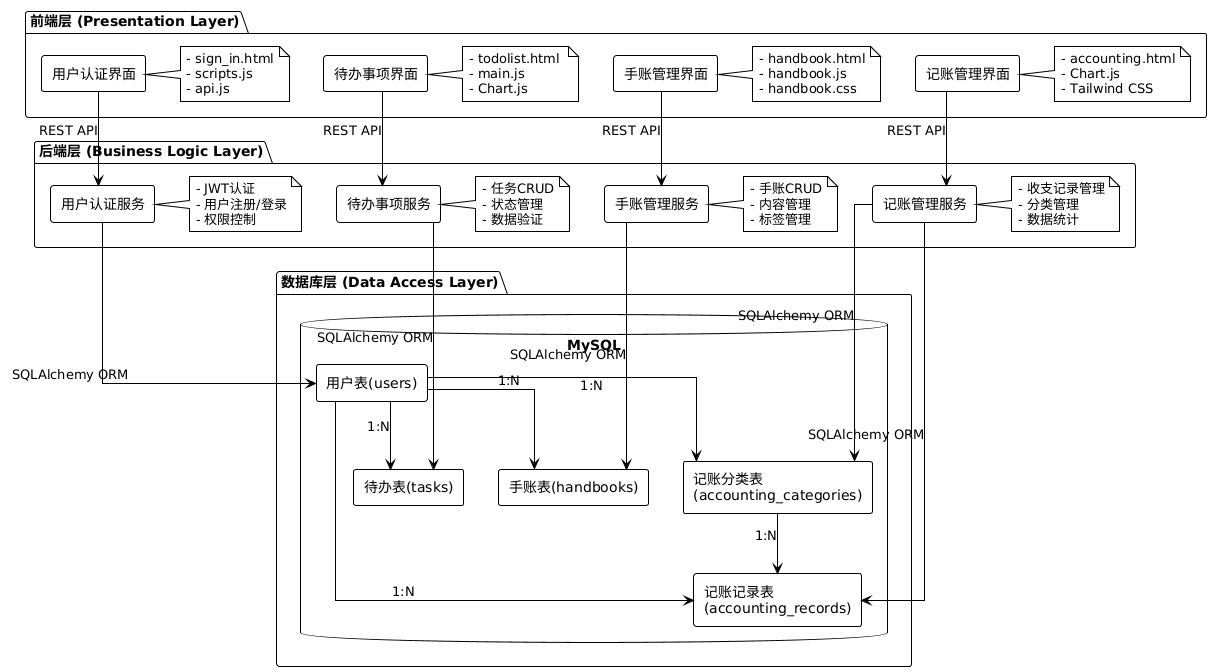
\includegraphics[width=0.8\textwidth]{img/architecture.png}
\caption{LifeMaster系统架构图}
\end{figure}

该架构具有以下优势:

\begin{itemize}
    \item \textbf{分层清晰}:各层职责明确,便于开发和维护
    \item \textbf{解耦合}:层与层之间通过标准接口通信,降低耦合度
    \item \textbf{可扩展}:可以独立扩展各层功能,不影响其他层
    \item \textbf{可维护}:便于定位问题和进行代码维护
\end{itemize}

\subsection{技术栈选择}

\subsubsection{前端技术栈}

\begin{table}[H]
\centering
\begin{tabular}{|l|l|p{6cm}|}
\hline
\textbf{技术} & \textbf{版本} & \textbf{用途} \\
\hline
HTML5 & - & 页面结构定义和语义化标记 \\
\hline
CSS3 & - & 样式设计和动画效果 \\
\hline
JavaScript & ES6+ & 页面交互逻辑和数据处理 \\
\hline
Tailwind CSS & 3.0+ & 响应式布局和组件样式 \\
\hline
Chart.js & 3.0+ & 数据可视化和图表展示 \\
\hline
Fetch API & - & 网络请求处理和数据交互 \\
\hline
\end{tabular}
\caption{前端技术栈}
\end{table}

\subsubsection{后端技术栈}

\begin{table}[H]
\centering
\begin{tabular}{|l|l|p{6cm}|}
\hline
\textbf{技术} & \textbf{版本} & \textbf{用途} \\
\hline
Python & 3.8+ & 后端开发语言 \\
\hline
Flask & 2.0+ & Web应用框架 \\
\hline
JWT & - & 身份认证和授权 \\
\hline
SQLAlchemy & 1.4+ & 对象关系映射(ORM)框架 \\
\hline
RESTful API & - & API设计规范 \\
\hline
\end{tabular}
\caption{后端技术栈}
\end{table}

\subsubsection{数据库技术}

\begin{table}[H]
\centering
\begin{tabular}{|l|l|p{6cm}|}
\hline
\textbf{技术} & \textbf{版本} & \textbf{用途} \\
\hline
MySQL & 8.0+ & 关系型数据库管理系统 \\
\hline
事务支持 & - & 保证数据一致性和完整性 \\
\hline
外键约束 & - & 维护数据引用完整性 \\
\hline
\end{tabular}
\caption{数据库技术栈}
\end{table}

\section{详细设计}

\subsection{前端层设计}

\subsubsection{模块划分}

前端采用模块化设计,按功能划分为不同的模块:

\textbf{前端项目结构:}
\begin{itemize}
    \item main.html - 主页面
    \item handbook.html - 手账模块页面
    \item accounting.html - 记账模块页面
    \item todolist.html - 待办模块页面
    \item sign\_in.html - 登录注册页面
    \item main.js - 主页面逻辑
    \item handbook.js - 手账模块逻辑
    \item accounting.js - 记账模块逻辑
    \item api.js - 前端API请求封装
    \item styles.css - 全局样式
    \item handbook.css - 手账模块样式
    \item 图片素材/ - 图片与字体等资源
    \item fonts/ - 字体文件
\end{itemize}

\subsubsection{关键设计决策}

\begin{enumerate}
    \item \textbf{模块化设计}:将不同功能的代码分离到独立文件中,提高代码的可维护性和可重用性
    
    \item \textbf{统一API接口层}:通过api.js文件统一处理所有后端通信,包括:
    \begin{itemize}
        \item 请求封装和响应处理
        \item 错误处理和重试机制
        \item 认证token管理
        \item 请求缓存策略
    \end{itemize}
    
    \item \textbf{响应式设计}:使用Tailwind CSS实现响应式布局,适配多种设备:
    \begin{itemize}
        \item 移动端:手机和小屏设备
        \item 平板端:中等屏幕设备
        \item 桌面端:大屏幕设备
    \end{itemize}
\end{enumerate}

\subsection{后端层设计}

\subsubsection{模块结构}

后端采用Flask框架的蓝图(Blueprint)模式进行模块化设计:

\textbf{后端项目结构:}
\begin{itemize}
    \item api/ - 后端API接口(Flask蓝图)
    \item api/index.py - API主入口
    \item migrations/ - 数据库迁移脚本
    \item test/ - 单元测试与数据库测试
    \item app.py - Flask应用入口
    \item requirements.txt - Python依赖
    \item Dockerfile - 容器部署配置
\end{itemize}

\subsubsection{关键设计决策}

\textbf{1. RESTful API设计}

API设计遵循RESTful规范,具有以下特点:

\begin{table}[H]
\centering
\begin{tabular}{|l|l|l|}
\hline
\textbf{HTTP方法} & \textbf{用途} & \textbf{示例} \\
\hline
GET & 获取资源 & GET /api/tasks \\
\hline
POST & 创建资源 & POST /api/tasks \\
\hline
PUT & 更新资源 & PUT /api/tasks/1 \\
\hline
DELETE & 删除资源 & DELETE /api/tasks/1 \\
\hline
\end{tabular}
\caption{RESTful API HTTP方法使用规范}
\end{table}

\textbf{2. 身份认证机制}

系统采用JWT(JSON Web Token)认证机制:

\begin{itemize}
    \item \textbf{Token生成}:用户登录成功后生成JWT token
    \item \textbf{Token验证}:每个API请求都需要验证token有效性
    \item \textbf{Token过期}:token过期时间设置为24小时
    \item \textbf{Token刷新}:提供token刷新机制,避免频繁重新登录
\end{itemize}

\textbf{3. 数据验证策略}

实施多层数据验证:

\begin{itemize}
    \item \textbf{请求参数验证}:验证参数类型、格式、长度等
    \item \textbf{业务规则验证}:验证业务逻辑的合理性
    \item \textbf{数据一致性检查}:确保数据库操作的一致性
\end{itemize}

\subsection{数据层设计}

\subsubsection{数据库表结构}

系统主要包含以下核心数据表:

\textbf{用户表(users)}

\texttt{CREATE TABLE users (}\\
\texttt{id VARCHAR(36) PRIMARY KEY,}\\
\texttt{username VARCHAR(50) NOT NULL,}\\
\texttt{email VARCHAR(120) UNIQUE NOT NULL,}\\
\texttt{password\_hash VARCHAR(128) NOT NULL,}\\
\texttt{created\_at DATETIME NOT NULL,}\\
\texttt{updated\_at DATETIME NOT NULL}\\
\texttt{);}

\textbf{待办表(tasks)}

\texttt{CREATE TABLE tasks (}\\
\texttt{id INTEGER PRIMARY KEY AUTO\_INCREMENT,}\\
\texttt{user\_id VARCHAR(36) NOT NULL,}\\
\texttt{text TEXT NOT NULL,}\\
\texttt{deadline DATETIME,}\\
\texttt{completed BOOLEAN DEFAULT FALSE,}\\
\texttt{created\_at DATETIME NOT NULL,}\\
\texttt{updated\_at DATETIME NOT NULL,}\\
\texttt{FOREIGN KEY (user\_id) REFERENCES users(id)}\\
\texttt{);}

\textbf{记账表(accounts)}

\texttt{CREATE TABLE accounts (}\\
\texttt{id INTEGER PRIMARY KEY AUTO\_INCREMENT,}\\
\texttt{user\_id VARCHAR(36) NOT NULL,}\\
\texttt{amount DECIMAL(10,2) NOT NULL,}\\
\texttt{category VARCHAR(50) NOT NULL,}\\
\texttt{description TEXT,}\\
\texttt{type ENUM('income', 'expense') NOT NULL,}\\
\texttt{date DATE NOT NULL,}\\
\texttt{created\_at DATETIME NOT NULL,}\\
\texttt{updated\_at DATETIME NOT NULL,}\\
\texttt{FOREIGN KEY (user\_id) REFERENCES users(id)}\\
\texttt{);}

\textbf{手账表(handbooks)}

\texttt{CREATE TABLE handbooks (}\\
\texttt{id INTEGER PRIMARY KEY AUTO\_INCREMENT,}\\
\texttt{user\_id VARCHAR(36) NOT NULL,}\\
\texttt{title VARCHAR(200) NOT NULL,}\\
\texttt{content TEXT,}\\
\texttt{images TEXT,}\\
\texttt{tags TEXT,}\\
\texttt{mood INTEGER,}\\
\texttt{date DATE NOT NULL,}\\
\texttt{created\_at DATETIME NOT NULL,}\\
\texttt{updated\_at DATETIME NOT NULL,}\\
\texttt{FOREIGN KEY (user\_id) REFERENCES users(id)}\\
\texttt{);}

\subsubsection{关键设计决策}

\textbf{1. 数据库选择}

选择MySQL作为主数据库的原因:

\begin{itemize}
    \item \textbf{ACID特性}:保证数据一致性和完整性
    \item \textbf{事务支持}:支持复杂的业务操作
    \item \textbf{外键约束}:维护数据引用完整性
    \item \textbf{成熟稳定}:广泛使用,文档完善,社区支持好
    \item \textbf{性能优秀}:适合中小型应用的性能需求
\end{itemize}

\textbf{2. ORM策略}

使用SQLAlchemy ORM框架的优势:

\begin{itemize}
    \item \textbf{对象映射}:将数据库表映射为Python对象
    \item \textbf{查询简化}:提供Pythonic的查询语法
    \item \textbf{连接管理}:自动管理数据库连接和连接池
    \item \textbf{迁移支持}:支持数据库版本管理和迁移
\end{itemize}

\section{安全设计}

\subsection{认证与授权}

\subsubsection{JWT Token认证机制}

系统采用JWT(JSON Web Token)进行用户认证:

\begin{table}[H]
\centering
\begin{tabular}{|l|p{10cm}|}
\hline
\textbf{组件} & \textbf{说明} \\
\hline
Header & 包含token类型和加密算法信息 \\
\hline
Payload & 包含用户ID、过期时间等claims信息 \\
\hline
Signature & 使用密钥对header和payload进行签名 \\
\hline
\end{tabular}
\caption{JWT Token结构}
\end{table}

\subsubsection{密码安全策略}

\begin{itemize}
    \item \textbf{密码加密}:使用bcrypt进行密码哈希存储
    \item \textbf{密码强度}:要求密码长度至少8位,包含字母和数字
    \item \textbf{防暴力破解}:登录失败次数限制和账户锁定机制
\end{itemize}

\subsection{数据安全}

\subsubsection{防注入攻击}

\begin{itemize}
    \item \textbf{SQL注入防护}:使用ORM参数化查询,避免直接拼接SQL
    \item \textbf{XSS防护}:对所有用户输入进行严格验证和过滤
    \item \textbf{CSRF防护}:为每个表单生成唯一的CSRF token
\end{itemize}

\section{性能优化}

\subsection{前端优化策略}

\subsubsection{资源优化}

\begin{table}[H]
\centering
\begin{tabular}{|l|p{8cm}|}
\hline
\textbf{优化策略} & \textbf{实现方式} \\
\hline
静态资源缓存 & 设置合适的Cache-Control头,使用版本号控制缓存更新 \\
\hline
按需加载 & 使用动态import()语法,实现代码分割和懒加载 \\
\hline
图片懒加载 & 使用Intersection Observer API实现图片懒加载 \\
\hline
资源压缩 & CSS/JS文件压缩,图片压缩和格式优化 \\
\hline
\end{tabular}
\caption{前端性能优化策略}
\end{table}

\subsection{后端优化策略}

\subsubsection{数据库优化}

\begin{table}[H]
\centering
\begin{tabular}{|l|p{8cm}|}
\hline
\textbf{优化策略} & \textbf{实现方式} \\
\hline
索引优化 & 为频繁查询的字段建立合适的索引,避免全表扫描 \\
\hline
查询缓存 & 使用Redis缓存热点数据和查询结果 \\
\hline
连接池管理 & 配置合适的数据库连接池大小,复用连接 \\
\hline
慢查询优化 & 监控和优化慢查询,使用EXPLAIN分析执行计划 \\
\hline
\end{tabular}
\caption{数据库性能优化策略}
\end{table}

\section{扩展性考虑}

\subsection{系统可扩展性}

\subsubsection{水平扩展}

\begin{itemize}
    \item \textbf{无状态设计}:应用服务器无状态,便于水平扩展
    \item \textbf{数据库分片}:支持数据库读写分离和分片策略
    \item \textbf{缓存集群}:使用Redis集群提供高可用缓存服务
    \item \textbf{CDN加速}:静态资源使用CDN分发,提高访问速度
\end{itemize}

\subsubsection{功能扩展}

\begin{itemize}
    \item \textbf{模块化设计}:新功能可以作为独立模块开发和部署
    \item \textbf{插件机制}:预留插件接口,支持第三方功能扩展
    \item \textbf{API版本管理}:支持API版本控制,保证向后兼容
    \item \textbf{微服务架构}:为未来微服务改造预留架构空间
\end{itemize}

\section{部署方案}

\subsection{环境要求}

\subsubsection{开发环境}

\begin{table}[H]
\centering
\begin{tabular}{|l|l|l|}
\hline
\textbf{组件} & \textbf{版本要求} & \textbf{说明} \\
\hline
Python & 3.8+ & 后端开发语言 \\
\hline
MySQL & 8.0+ & 数据库服务 \\
\hline
Node.js & 14+ & 前端构建工具(用于前端构建) \\
\hline
Redis & 6.0+ & 缓存服务(可选) \\
\hline
\end{tabular}
\caption{开发环境要求}
\end{table}

\subsubsection{生产环境}

\begin{table}[H]
\centering
\begin{tabular}{|l|l|l|}
\hline
\textbf{组件} & \textbf{配置要求} & \textbf{说明} \\
\hline
CPU & 2核心+ & 推荐4核心以上 \\
\hline
内存 & 4GB+ & 推荐8GB以上 \\
\hline
存储 & 50GB+ & SSD推荐 \\
\hline
网络 & 10Mbps+ & 稳定的网络连接 \\
\hline
\end{tabular}
\caption{生产环境配置要求}
\end{table}

\subsection{部署步骤}

\subsubsection{数据库初始化}

\begin{enumerate}
    \item 创建数据库:CREATE DATABASE lifemaster;
    \item 创建用户:CREATE USER 'lifemaster'@'localhost' IDENTIFIED BY 'password';
    \item 授权:GRANT ALL PRIVILEGES ON lifemaster.* TO 'lifemaster'@'localhost';
    \item 执行数据库迁移:python -m flask db upgrade
\end{enumerate}

\subsubsection{后端服务部署}

\begin{enumerate}
    \item 安装依赖:pip install -r requirements.txt
    \item 配置环境变量:设置FLASK\_APP、DATABASE\_URL等
    \item 启动服务:gunicorn -w 4 -b 0.0.0.0:5000 app:app
\end{enumerate}

\subsubsection{前端资源部署}

\begin{enumerate}
    \item 构建前端资源:npm install \&\& npm run build
    \item 部署到Web服务器:cp -r dist/* /var/www/html/
    \item 配置Nginx:配置反向代理和静态资源服务
\end{enumerate}

\subsubsection{Nginx配置}

Nginx作为反向代理服务器,负责:
\begin{itemize}
    \item 前端路由处理
    \item API请求代理到后端服务
    \item 静态资源缓存
    \item SSL/TLS终止
\end{itemize}

\section{总结}

本文档详细阐述了LifeMaster系统的架构设计,涵盖了系统概述、架构设计、详细设计、安全设计、性能优化、扩展性考虑和部署方案等各个方面。

\subsection{架构优势}

LifeMaster系统架构具有以下主要优势:

\begin{itemize}
    \item \textbf{分层清晰}:三层架构职责明确,便于开发和维护
    \item \textbf{技术成熟}:选择了经过验证的成熟技术栈
    \item \textbf{安全可靠}:完善的安全防护机制和数据保护措施
    \item \textbf{性能优秀}:多层次的性能优化策略
    \item \textbf{易于扩展}:模块化设计便于功能扩展和技术升级
    \item \textbf{运维友好}:提供完整的部署和监控方案
\end{itemize}

\subsection{设计原则}

在架构设计过程中,我们始终遵循以下设计原则:

\begin{itemize}
    \item \textbf{简单性}:保持架构简单清晰,避免过度设计
    \item \textbf{可维护性}:代码结构清晰,便于维护和调试
    \item \textbf{可扩展性}:预留扩展空间,支持业务增长
    \item \textbf{可靠性}:确保系统稳定运行,数据安全可靠
    \item \textbf{性能性}:优化系统性能,提供良好用户体验
\end{itemize}

此架构文档将作为系统开发、部署和维护的重要参考,为项目的成功实施提供技术保障。

\label{LastPage}
\end{document}
